


\documentclass{article}
\usepackage[utf8]{inputenc}

%\usepackage[md]{titlesec}
\usepackage{graphicx}

\usepackage{blindtext}

\usepackage[export]{adjustbox}
\usepackage{color}
\usepackage{hyperref} %% Enable hyperref links from toc
\hypersetup{
    colorlinks,
    citecolor=black,
    filecolor=black,
    linkcolor=blue,
    urlcolor=black
}

\usepackage{subcaption} % Enables subcaption

\usepackage{listings}

% Sets the depth of toc to be limited to sections
\setcounter{tocdepth}{3} 



%% Changes the subsubsection to be numbered with alphabets
 \renewcommand{\thesubsection}{\alph{subsection}}
\renewcommand{\thesubsubsection}{\roman{subsubsection}}


%Add path to images
%\graphicspath{./imgs/}

\date{November 11, 2016}


\title{\textbf{Assignment 11}\\Configuring Security and Access-Lists on Cisco Devices and
Simulating Infrastructure Attacks}

\author{Siddhartha Pandey (s316620)}

\begin{document}

\maketitle
\newpage
\tableofcontents
\newpage

\part{Introduction}

The purpose of this assignment is to learn how to secure Cisco devices and how to configure an access list on the routers, which is basically a firewall. To complete the assignment you need to have Cisco Packet Tracer installed on your system. 

\part{Methods and Materials}


\section{Security Measures}

\subsection{Deploying the routers and the switch}

We use the 1841 model when deploying the router and the model 2960-24TT for the switch. We deploy both the routers and the switch in Packet Tracer. 


\subsection{Configuring Passwords}
After deploying the router and the switch, we start configuration for the router. We use the \textbf{enable} command to enter the privileged EXEC mode, then the \textbf{configure terminal} command to enter the configuration mode. We add security to the router by configuring a password. We use the command \textbf{enable secret \textless\emph{your password}\textgreater} to enable the password, where \emph{your password} is replaced with the actual password. There is two ways to configure the password to access the router's priveleged EXEC mode. We can either use the \textbf{enable secret} or the \textbf{enable password} command. The \textit{enable secret} takes precedence over the \textit{enable password} command.

\subsubsection{\emph{enable password}}
The \textit{enable secret} command sets a password for the various privilege levels. We use the command \textbf{enable password \textless\emph{password}\textgreater} to set the password. This command does not encrypt the password saved in the \emph{running-config} file.

\subsubsection{\emph{enable secret}}
The \textit{enable secret}  command establishes a password for the privilege levels. The difference to the \textit{enable password} is that this command encrypts the password stored in the \emph{running-config} file providing better security.

\subsection{Observing the changes with password enabled}

After we issue the \textbf{enable secret} command we have to enter the password when going from the user EXEC mode to the priveleged EXEC mode, we can this in Figure \ref{fig:passprev}. 

\begin{figure}
\centering
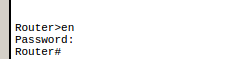
\includegraphics[width=0.5\textwidth]{imgs/passprev.png}
\caption{Entering the privelege EXEC mode with password enable with \textbf{enable secret} command.}
\label{fig:passprev}
\end{figure}

\subsection{Storing password in \emph{running-config}}
We can see the \textit{running-config} using the \textbf{show running-config} command in the CLI of the router. We can observe as seen in Figure \ref{fig:runconfpass} that the password is encrypted.

\begin{figure}[h]
    \centering
    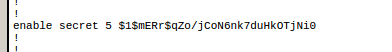
\includegraphics[width=0.8\textwidth]{imgs/runconfpass}
    \caption{The \textit{running-config} in router, storing the password after \textbf{enable secret} command.}
    \label{fig:runconfpass}
\end{figure}


The 5 that follows after \textit{enable secret} implies that the following is a hash for the password, encrypted using MD5 algorithm. We can see this in Figure \ref{fig:ensec5}, there is an encrypted hash of the password following the 5. 

\begin{figure}[h]
    \centering
    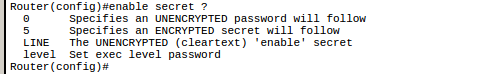
\includegraphics[width=0.9\textwidth]{imgs/ensec5}
    \caption{Checking \textit{enable secret} options}
    \label{fig:ensec5}
\end{figure}

\subsubsection{Extra}

We can use both the \textbf{enable secret} and the \textbf{enable password} command at the same time. The router uses the encrypted password when both are present. When using the same password for both the encrypted and the unencrypted password, the CLI warns us to use different but still allows it as seen in Figure \ref{fig:enpassonly}.

\begin{figure}[h]
    \centering
    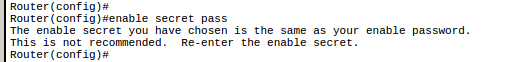
\includegraphics[width=\textwidth]{imgs/enpassonly}
    \caption{Using the same password for both \textbf{enable secret} and \textbf{enable password}}
    \label{fig:enpassonly}
\end{figure}

\subsection{Enable password for console access}

Then we will also configure a password for the console access. We use the commands \textbf{line  con 0} in the configuration mode. This lets us configure the primary terminal line. 
\subsubsection{Set password}
Then we use the \textbf{password} command to set the password.
\subsubsection{Enable login for console access}
We use the \textbf{login} command to enable password checking. 

\subsubsection{Loggin prompt}
After setting the password for console access we get prompted to enter the password when we open the CLI, we need to enter the password even to enter the user EXEC mode as can be seen in Figure \ref{fig:logincon}.

\begin{figure}[h]
    \centering
    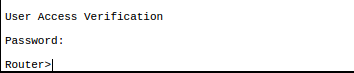
\includegraphics[width=0.7\textwidth]{imgs/logincon}
    \caption{Login prompt for access to the console.}
    \label{fig:logincon}
\end{figure}

\subsection{Console Access Password in \emph{running-conf}}

The password set for console access is not encrypted when we check the \textit{running-configuration} using \textbf{show running-conf}, the password is stored in plain text. 

\subsection{configuring password for telnet}


We enter the telnet configuration mode using the \textbf{line vty 0 4} command in the global configuration mode.


We then set the password with the \textbf{password} command and enable login using the \textbf{login} command. 

Checking the \textit{running-configuration} we can see that the passwords for the \textit{console access} and the \textit{terminal access} are stored in plain text.

\subsection{Encrypt all passwords}

As many of the passwords are stored in plain text we need to increase the security of the plain-text password. We use the \textbf{service password-encryption} command in the global configuration mode to encrypt all the unencrypted passwords. 

\subsubsection{\textit{running-conf} after encrypting password}

We can see in Figure \ref{fig:encpasses} that all the password have been encrypted. We can see that there is a number, 7, after password. This specifies that this was encryption Type 7.  

\begin{figure}[h]
    \centering
    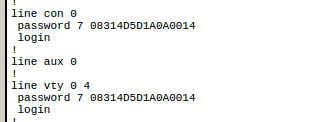
\includegraphics[width=0.6\textwidth]{imgs/encpasses}
    \caption{The encrypted password after running \textbf{service password-encryption}}
    \label{fig:encpasses}
\end{figure}

\subsection{Type 5 and Type 7 encryptions}

As seen in Figure \ref{fig:encpasses} all the passwords that were encrypted using the \textbf{service password-encryption} command was encrypted with encryption Type 7. Previously when running the \textbf{enable secret} command the passwords were encrypted using Type 5, as seen in Figure \ref{fig:runconfpass}.

The Type 5 encryption is done using an MD5 algorithm to generate the password hash. Whereas the Type 7 encryption is done using a weak algorithm, it is just XORs the password.

\subsection{Securing the Switch}

We follow the same procedures to secure the switch by adding password and encrypting them. We use the same password as in the previous assignment.

\begin{itemize}
    \item \textbf{enable secret} Add password for accessig the privileged EXEC mode.
    \item \textbf{line con 0} Configure console access 
        \subitem \textbf{password} Set password for console access
        \subitem \textbf{login} Enable password login for console access
    \item \textbf{line vty 0 4} Configure telnet access
        \subitem \textbf{password} Set password for telnet access
        \subitem \textbf{login} Enable password login for telnet access
     \item \textbf{service password-encryption} Encrypt all pasword in the \textit{runnnig-config}
\end{itemize}

\section{Configuring Access lists}


\subsection{Setting up the topology}

We use 4 like the router previously configured and connect them to the switch that was previously configured. Our topology in Packet Tracer looks like Figure \ref{fig:2topo}.

\begin{figure}[h]
\centering
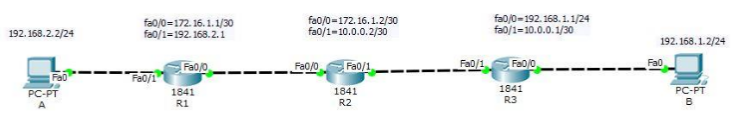
\includegraphics[width=0.7\textwidth]{imgs/2topo}
\caption{Topology in Packet Tracer}
\label{fig:2topo}
\end{figure}

\subsection{Configuring the devices with IP addresses}

Now that we have a topology in Packet Tracer, we will configure the all the interfaces with an IP address as seen in Table \ref{tab:2intip}. After all the interfaces have been assigned an IP address we will make sure that the interfaces are \textit{up}. We will also configure the default gateway for the hosts to be the interface of the router they are each connected to respectively.

\begin{table}[h]
\centering
\begin{tabular}{|c|c|c|}
\hline
Device Name & Interface & IP Address \\
\hline
Router0 & Fa0/0 & 10.0.0.1/24 \\
Router 1 & Fa0/0 &  10.0.0.2/24\\
Router 2 & Fa0/0 & 10.0.0.3/24\\
Router 3 & Fa0/0 & 10.0.0.4/24\\
Router0 & Fa0/1 & 192.168.0.1/24\\
Router1 & Fa0/1 & 192.168.1.1/24\\
Router2 & Fa0/1 & 192.168.2.1/24\\
Router3 & Fa0/1 & 192.168.3.1/24\\
PC0 & Fa0/0 & 192.168.0.2/24\\
PC1 & Fa0 & 192.168.1.2/24\\
PC2 & Fa0 & 192.168.2.2/24\\
PC3 & Fa0 & 192.168.3.2/24\\
\hline
\end{tabular}
\caption{Interface IP addresses for hosts and routers.}
\label{tab:2intip}
\end{table}


\subsection{Checking connectivity}

We check the connectivity of the network to verify that everything is configured properly. The routers in the 10.0.0.0/24 network should ping each other as seen in Figure \ref{fig:2pingrouters}, and the PC should be able to ping its own router  \ref{fig:2pingdef}. 

\begin{figure}[h]
\centering
\includegraphics[width=0.6\textwidth]{imgs/2pingrouters}
\caption{Checking connectivity between routers.}
\label{fig:2pingrouters}
\end{figure}

\begin{figure}[h]
\centering
\includegraphics[width=0.6\textwidth]{imgs/2pingdef}
\caption{Checking connectivity between the hosts and the routers.}
\label{fig:2pingdef}
\end{figure}

\subsection{Configuring Routing with RIPv2}

For full connectivity in the network we will configure the routers with a routing protocol. Here, the RIPv2 routing protocol will be used. We configure the routing protocol by issuing the following commands:
\begin{itemize}
    \item \textbf{router rip} In the configuration mode.
    \subitem \textbf{version 2} Specifies the routing protocol as RIP version 2
    \subitem \textbf{network x.x.x.x} This command is issued for all the networks that are connected to the router, where x.x.x.x is one specific network.
\end{itemize}


We use this method to configure all the routers in the topology. Then check that there is connectivity between all the hosts. We can see in Figure \ref{fig:pinghosts} that there is full connectivity between the hosts. 

\begin{figure}[h]
\centering
\includegraphics[width=0.6\textwidth]{imgs/pinghosts}
\caption{Checking connectivity between hosts}
\label{fig:pinghosts}
\end{figure}

\subsection{Configuring ACL}

Now we wil configure ACLs in our routers. Now we want to allow all traffic originating from the students and system administrator network to reach the professor's network, but we do not want to let the school employees access the professor's network. To do this we deploy an access-list on Router1 on all the incoming traffic on interface Fa0/0. We do this by create two rules with standard ACL that allows the traffic of networks 192.168.0.0/24 and 192.168.3.0/24. We do this using the following commands, in the global configuration mode: 
\begin{itemize}
\item \textbf{access-list 1 permit 192.168.0.0 0.0.0.255}
\item \textbf{access-list 1 permit 192.168.3.0 0.0.0.255}
\end{itemize}
Then we add this two rules to the interface Fa0/0 by using the command:\\
\begin{itemize}
\item \textbf{ip access-group 1 in}
\end{itemize}
This specifies that it allows incoming traffic of access-group 1 (defined above) only at interface Fa0/0 at Router1. When checking connectivity with \textit{ping} we can see that this will let PC0 and PC3 reach PC1, but not PC2 as seen in Figure \ref{fig:2aclping2}.

\begin{figure}[h]
\centering
\includegraphics[width=0.6\textwidth]{imgs/2aclping2}
\caption{Checking connectivity from PC0, PC2 and PC3 to PC1}
\label{fig:2aclping2}
\end{figure}

We can not ping even from any of the other routers. After letting some time pass there will be no connectivity between any of the hosts as the routing table at Router1 will not be updated as only the student and system administrator's networks traffic is recieved by the interface Fa0/0 at Router1, we can see that in Figure \ref{fig:router1rt}. An alternative would be to configure the access-list groups at Fa0/1 and restrict incoming outgoing traffic. So the packets can be recieved by the router but would be droped before it went to PC1. The command to use would be : \textbf{ip access-group 1 out} at interface Fa0/1 in Router1. Another alternative would be to add the network 10.0.0.0/24 to access-list for inbound, though this will also allow the routers to reach the professors network (PC1).

\begin{figure}[h]
\centering
\includegraphics[width=0.8\textwidth]{imgs/router1rt}
\caption{Routing table at Router1}
\label{fig:router1rt}
\end{figure}

\subsection{Configuring outbound ACL}
Now configuring an outbound ACL that permits all traffic originating from the professors network.  We make an access-list with number2 with the command:
\begin{itemize}
\item \textbf{access-list 1 permit 192.168.1.0 0.0.0.255}
\end{itemize}
And then add this access-list to the internal interface Fa0/1 at Router1. We do this using the command: 
\begin{itemize}
\item \textbf{ip access-group 2 in}
\end{itemize}


I can ping from PC1 to PC0 and PC3, but only if I implement one of alternative methods, for restricting access to PC2, as mentioned above.

\subsection{Extended ACLs}

Extended ACLs can specify some special reserved keywords, One one of the keyword is \textit{any} which corressponds to 0.0.0.0/255.255.255.255, another is \textit{host} which is same as typing ``/0.0.0.0''. The extended ACLs use higher numbers (100-199) whereas standard ACLs use lower numbers (1-99). 

\subsection{Allowing only ICMP traffic}

With extended ACLs we can restrict traffic to only ICMP traffic, or any other particular protocol, useing the command: 
\begin{itemize}
\item \textbf{access-list 101 permit icmp any any}
\end{itemize}  And setting the rules to both the interfaces of a router. 

\subsection{Allowign only a particular host external access}

We can give access to only 1 PC from the school employee network to have access to students network by allowing traffic going only from that host to the students network. We make a rule that looks like:\\
\begin{itemize}
\item \textbf{access-list 101 permit ip host 192.168.2.2 192.168.0.0 0.0.0.255}
\end{itemize}

\end{document}








